\section{Theory}

Light propagates through a medium at a lower velocity than in vaccum. This is described by the index of refraction of the medium

\begin{equation}
  \label{eq:refrInd}
  n = \frac{c_0}{v},
\end{equation}

where $c_0$ is the speed of light in vaccum and $v$ is the velocity in the medium\cite{phH}. By this one can define the optical path length (OPL) as the length the light experiences, that is if the light propagates through a medium of length $L$ and refractive index $n$, then the OPD will be

\begin{equation*}
  \tn{OPD} = nL.
\end{equation*}

The refractive index is thus a measure of how dense a material is and must therefore be proportional to the pressure. Namely by increasing the pressure $P$ from vaccum, then

\begin{equation}
  \label{eq:refrVaccum}
  n-1 = \alpha \frac{\Delta P}{P_{atm}},
\end{equation}

where $P_{atm}$ is the atmospheric pressure and $\alpha$ is the proportionality constant. Note thet since $P$ is measured from vaccum then $\alpha=n-1$ at atmospheric pressure.

\subsection{The Michelson Interferometer}
A Michelson interferometer consists of a laser beam being splitted into a reference leg $L_1$ and a signal leg $L_2$. The beams are then reflected back and reassembled at a sensor. A schematic sketch of this is found in Fig. \ref{fig:michelsonInterferometer}. If the beams are aligned correctly they will interfere with eachocher and constructive interference will occur if

\begin{equation}
\label{eq:interference}
  \tn{OPD} = N \lambda,
\end{equation}

where OPD is the optical path difference between the legs, $N$ is an integer and $\lambda$ is the wavelength of the light.

\begin{figure}[H]
  \centering
  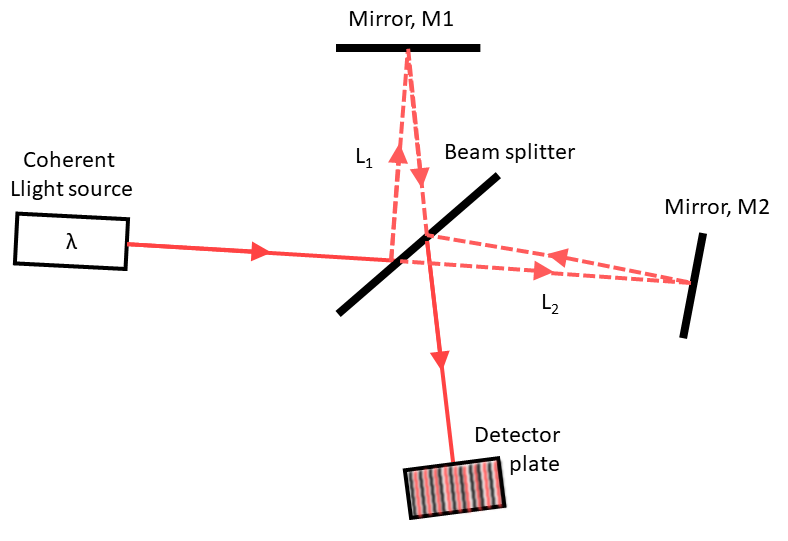
\includegraphics[width=0.8\textwidth]{Method.png}
  \caption{Principle of michelson interferometer. A coherent light source is split into two individual rays, these rays are reflected onto two mirrors and joined togheter again. When aligned propertly an interference pattern can be observed at a detector plate.}
  \label{fig:michelsonInterferometer}
\end{figure}

\subsection{Method}

If a gas chamber of length $d$ is put on the sensor leg as shown in Fig. \ref{fig:experimentalSetup} the the OPD can be found as

\begin{equation}
  \label{eq:OPD}
  \tn{OPD} = 2\tn{OPL}_{L_2} - 2\tn{OPL}_{L_1} = 2nd + \tn{const.}
\end{equation}

Using the interference condition Eq. \eqref{eq:interference} this can be reduced to

\begin{equation*}
  N \lambda = 2nd + \tn{const.}.
\end{equation*}

Instead of counting the absolute number of interference maxima, called fringes, one can count the number of fringes that appear when changing the refractive index of the sample. This can then be rewritten as

\begin{equation}
\label{eq:delta}
  \Delta N \lambda = 2d \Delta n.
\end{equation}

If one measures this from vaccum one can make us of Eq. \eqref{eq:refrVaccum} in Eq. \eqref{eq:delta} and obtain

\begin{equation}
\label{eq:slope}
  \Delta N = \frac{2d\alpha}{\lambda P_{atm}} \Delta P.
\end{equation}

Thus, by continuously increasing the pressure of a gas from vaccum and counting how many fringes that has passed a sensor one can find the refractive index from the slope of Eq. \eqref{eq:slope} and $n=\alpha+1$.
